\documentclass{article}\usepackage[]{graphicx}\usepackage[]{color}
% maxwidth is the original width if it is less than linewidth
% otherwise use linewidth (to make sure the graphics do not exceed the margin)
\makeatletter
\def\maxwidth{ %
  \ifdim\Gin@nat@width>\linewidth
    \linewidth
  \else
    \Gin@nat@width
  \fi
}
\makeatother

\definecolor{fgcolor}{rgb}{0.345, 0.345, 0.345}
\newcommand{\hlnum}[1]{\textcolor[rgb]{0.686,0.059,0.569}{#1}}%
\newcommand{\hlstr}[1]{\textcolor[rgb]{0.192,0.494,0.8}{#1}}%
\newcommand{\hlcom}[1]{\textcolor[rgb]{0.678,0.584,0.686}{\textit{#1}}}%
\newcommand{\hlopt}[1]{\textcolor[rgb]{0,0,0}{#1}}%
\newcommand{\hlstd}[1]{\textcolor[rgb]{0.345,0.345,0.345}{#1}}%
\newcommand{\hlkwa}[1]{\textcolor[rgb]{0.161,0.373,0.58}{\textbf{#1}}}%
\newcommand{\hlkwb}[1]{\textcolor[rgb]{0.69,0.353,0.396}{#1}}%
\newcommand{\hlkwc}[1]{\textcolor[rgb]{0.333,0.667,0.333}{#1}}%
\newcommand{\hlkwd}[1]{\textcolor[rgb]{0.737,0.353,0.396}{\textbf{#1}}}%
\let\hlipl\hlkwb

\usepackage{framed}
\makeatletter
\newenvironment{kframe}{%
 \def\at@end@of@kframe{}%
 \ifinner\ifhmode%
  \def\at@end@of@kframe{\end{minipage}}%
  \begin{minipage}{\columnwidth}%
 \fi\fi%
 \def\FrameCommand##1{\hskip\@totalleftmargin \hskip-\fboxsep
 \colorbox{shadecolor}{##1}\hskip-\fboxsep
     % There is no \\@totalrightmargin, so:
     \hskip-\linewidth \hskip-\@totalleftmargin \hskip\columnwidth}%
 \MakeFramed {\advance\hsize-\width
   \@totalleftmargin\z@ \linewidth\hsize
   \@setminipage}}%
 {\par\unskip\endMakeFramed%
 \at@end@of@kframe}
\makeatother

\definecolor{shadecolor}{rgb}{.97, .97, .97}
\definecolor{messagecolor}{rgb}{0, 0, 0}
\definecolor{warningcolor}{rgb}{1, 0, 1}
\definecolor{errorcolor}{rgb}{1, 0, 0}
\newenvironment{knitrout}{}{} % an empty environment to be redefined in TeX

\usepackage{alltt}
\title{Statistical Programming with R\\Assignment 2}

\author{\small Tove Henning\\ \small Carl Munkby\\ \small Johannes Zetterberg}
\date{}

\usepackage[margin = 1in]{geometry}
\IfFileExists{upquote.sty}{\usepackage{upquote}}{}
\begin{document}
\maketitle

\pagebreak


\begin{knitrout}
\definecolor{shadecolor}{rgb}{0.969, 0.969, 0.969}\color{fgcolor}\begin{kframe}
\begin{alltt}
\hlkwd{library}\hlstd{(StatProg)}
\hlkwd{library}\hlstd{(ggplot2)}

\hlcom{#### OLS}
\hlstd{olsFun} \hlkwb{<-} \hlkwa{function}\hlstd{(}\hlkwc{data}\hlstd{)\{}
  \hlcom{### set column names and add intercept column to X}
  \hlstd{Y} \hlkwb{<-} \hlstd{data[,}\hlnum{1}\hlstd{]}
  \hlstd{N} \hlkwb{<-} \hlkwd{nrow}\hlstd{(data)}
  \hlstd{X} \hlkwb{<-} \hlkwd{cbind}\hlstd{(}\hlkwd{rep}\hlstd{(}\hlnum{1}\hlstd{, N), data[,}\hlnum{2}\hlstd{])}

  \hlcom{### calculate the formel and extract the Beta coefficient }
  \hlstd{beta_ols}\hlkwb{=}\hlstd{(}\hlkwd{solve}\hlstd{(}\hlkwd{t}\hlstd{(X)}\hlopt \hlstd{X)} \hlopt \hlstd{(}\hlkwd{t}\hlstd{(X)} \hlopt \hlstd{Y))[}\hlnum{2}\hlstd{,}\hlnum{1}\hlstd{]}

  \hlkwd{return}\hlstd{(beta_ols)}
\hlstd{\}}

\hlcom{#Här är en kommentar om OLS. blabla bla blabakljdgklajkl}

\hlstd{testData} \hlkwb{<-} \hlkwd{cbind}\hlstd{(} \hlkwd{c}\hlstd{(}\hlnum{0.62}\hlstd{,} \hlnum{0.18}\hlstd{,} \hlnum{3.92}\hlstd{,} \hlnum{0.80}\hlstd{,} \hlopt{-}\hlnum{5.15}\hlstd{),}
\hlkwd{c}\hlstd{(}\hlnum{0.44}\hlstd{,} \hlnum{1.49}\hlstd{,} \hlnum{0.69}\hlstd{,} \hlnum{0.13}\hlstd{,} \hlnum{1.90}\hlstd{) )}

\hlkwd{olsFun}\hlstd{(}\hlkwc{data} \hlstd{= testData)}
\end{alltt}
\begin{verbatim}
## [1] -3.092464
\end{verbatim}
\end{kframe}
\end{knitrout}

\begin{knitrout}
\definecolor{shadecolor}{rgb}{0.969, 0.969, 0.969}\color{fgcolor}\begin{kframe}
\begin{alltt}
\hlcom{##### weighted least squares}
\hlstd{wlsFun} \hlkwb{<-} \hlkwa{function}\hlstd{(}\hlkwc{data}\hlstd{,} \hlkwc{lambda}\hlstd{)\{}
  \hlkwa{if} \hlstd{(}\hlkwd{is.numeric}\hlstd{(lambda)}\hlopt{==}\hlnum{FALSE}\hlstd{)\{}\hlkwd{print}\hlstd{(}\hlstr{"lambda is not numeric"}\hlstd{) \}}
  \hlkwa{else}\hlstd{\{}
    \hlcom{### create variable for the number of observations in the dataset}
    \hlstd{N} \hlkwb{<-} \hlkwd{nrow}\hlstd{(data)}

    \hlcom{### set column names and add intercept column for X}
    \hlstd{Y} \hlkwb{<-} \hlstd{data[,}\hlnum{1}\hlstd{]}
    \hlstd{X} \hlkwb{<-} \hlkwd{cbind}\hlstd{(}\hlkwd{rep}\hlstd{(}\hlnum{1}\hlstd{,N), data[,}\hlnum{2}\hlstd{])}

    \hlcom{### create a zero matrix N x N}
    \hlstd{Z} \hlkwb{<-} \hlkwd{matrix}\hlstd{(}\hlnum{0}\hlstd{, N, N)}

    \hlcom{## make a forloop to put in the error terms on the diagonal }
    \hlcom{## to create the error covariance matrix}
    \hlstd{er} \hlkwb{<-} \hlkwa{NULL}
    \hlkwa{for} \hlstd{(i} \hlkwa{in} \hlnum{1}\hlopt{:}\hlstd{N) \{}
      \hlstd{er[i]} \hlkwb{<-} \hlkwd{exp}\hlstd{(X[i,}\hlnum{2}\hlstd{]}\hlopt{*}\hlstd{lambda)}
      \hlstd{Z[i,i]} \hlkwb{<-} \hlstd{er[i]}
    \hlstd{\}}
    \hlcom{### calculate and extract the Beta coefficient}
    \hlstd{beta_wls} \hlkwb{=} \hlstd{((}\hlkwd{solve}\hlstd{(}\hlkwd{t}\hlstd{(X)}\hlopt\hlstd{(}\hlkwd{solve}\hlstd{(Z))}\hlopt\hlstd{X)}\hlopt\hlkwd{t}\hlstd{(X)}\hlopt
                   \hlstd{(}\hlkwd{solve}\hlstd{(Z))}\hlopt\hlstd{Y))[}\hlnum{2}\hlstd{,}\hlnum{1}\hlstd{]}
  \hlkwd{return}\hlstd{(beta_wls)}
  \hlstd{\}}
\hlstd{\}}

\hlkwd{wlsFun}\hlstd{(}\hlkwc{data} \hlstd{= testData,} \hlkwc{lambda} \hlstd{=} \hlnum{2}\hlstd{)}
\end{alltt}
\begin{verbatim}
## [1] 0.007392226
\end{verbatim}
\end{kframe}
\end{knitrout}

\begin{knitrout}
\definecolor{shadecolor}{rgb}{0.969, 0.969, 0.969}\color{fgcolor}\begin{kframe}
\begin{alltt}
\hlcom{#### FWLS}
\hlcom{# H<U+653C><U+3E34>r g<U+663C><U+3E36>r jag lite kommentarer }
\hlcom{# Bla bla bla}
\hlstd{fwlsFun} \hlkwb{<-} \hlkwa{function}\hlstd{(}\hlkwc{data}\hlstd{,} \hlkwc{trueVar}\hlstd{)\{}
  \hlstd{y} \hlkwb{=} \hlstd{data[,}\hlnum{1}\hlstd{]}
  \hlstd{N} \hlkwb{<-} \hlkwd{nrow}\hlstd{(data)}
  \hlstd{X} \hlkwb{=} \hlkwd{cbind}\hlstd{(}\hlkwd{rep}\hlstd{(}\hlnum{1}\hlstd{,N), data[,}\hlnum{2}\hlopt{:}\hlkwd{ncol}\hlstd{(data)])}

  \hlstd{mod} \hlkwb{=} \hlkwd{lm}\hlstd{(y} \hlopt{~ -}\hlnum{1} \hlopt{+}\hlstd{X)}
  \hlstd{res} \hlkwb{=} \hlstd{mod}\hlopt{$}\hlstd{residuals}
  \hlstd{res2} \hlkwb{=} \hlstd{res}\hlopt{^}\hlnum{2}

  \hlstd{ln_res2} \hlkwb{=} \hlkwd{lm}\hlstd{(}\hlkwd{log}\hlstd{(res2)} \hlopt{~  -}\hlnum{1} \hlopt{+}\hlstd{X)}
  \hlstd{lambda_hat} \hlkwb{=} \hlstd{ln_res2}\hlopt{$}\hlstd{coefficients[}\hlnum{2}\hlstd{]}

  \hlkwa{if}\hlstd{(trueVar} \hlopt{==} \hlnum{TRUE}\hlstd{)\{}
    \hlstd{error_cov} \hlkwb{=} \hlkwd{matrix}\hlstd{(}\hlnum{0}\hlstd{, N, N)}
    \hlkwa{for}\hlstd{(i} \hlkwa{in} \hlnum{1}\hlopt{:}\hlstd{N)\{}
      \hlstd{error_cov[i,i]} \hlkwb{<-} \hlkwd{exp}\hlstd{(X[i,}\hlnum{2}\hlstd{]}\hlopt{*}\hlstd{lambda_hat)}
    \hlstd{\}}

  \hlstd{\}}
  \hlkwa{else if}\hlstd{(trueVar} \hlopt{==} \hlnum{FALSE}\hlstd{)}
  \hlstd{\{}
    \hlstd{error_cov} \hlkwb{=} \hlkwd{matrix}\hlstd{(}\hlnum{0}\hlstd{, N, N)}
    \hlkwa{for}\hlstd{(i} \hlkwa{in} \hlnum{1}\hlopt{:}\hlstd{N)\{}
      \hlstd{error_cov[i,i]} \hlkwb{<-} \hlnum{1} \hlopt{+} \hlstd{X[i,}\hlnum{2}\hlstd{]}\hlopt{*}\hlstd{lambda_hat}
    \hlstd{\}}

  \hlstd{\}}
\hlstd{beta_fwls} \hlkwb{=} \hlstd{(}\hlkwd{solve}\hlstd{(}\hlkwd{t}\hlstd{(X)}\hlopt\hlkwd{solve}\hlstd{(error_cov)}\hlopt\hlstd{X)}\hlopt\hlkwd{t}\hlstd{(X)}\hlopt\hlkwd{solve}\hlstd{(error_cov)}\hlopt\hlstd{y)[}\hlnum{2}\hlstd{,}\hlnum{1}\hlstd{]}

\hlkwd{return}\hlstd{(beta_fwls)}
\hlstd{\}}
\hlkwd{fwlsFun}\hlstd{(}\hlkwc{data} \hlstd{= testData,} \hlkwc{trueVar} \hlstd{=} \hlnum{TRUE}\hlstd{)}
\end{alltt}
\begin{verbatim}
## [1] -2.615266
\end{verbatim}
\begin{alltt}
\hlkwd{fwlsFun}\hlstd{(}\hlkwc{data} \hlstd{= testData,} \hlkwc{trueVar} \hlstd{=} \hlnum{FALSE}\hlstd{)}
\end{alltt}
\begin{verbatim}
## [1] -2.750474
\end{verbatim}
\end{kframe}
\end{knitrout}


First we created the OLS fun to...

\begin{knitrout}
\definecolor{shadecolor}{rgb}{0.969, 0.969, 0.969}\color{fgcolor}\begin{kframe}
\begin{alltt}
\hlcom{#### Data simulation}
\hlstd{DataFun} \hlkwb{<-} \hlkwa{function}\hlstd{(}\hlkwc{n}\hlstd{,} \hlkwc{lambda}\hlstd{) \{}

    \hlcom{# independent variable}
    \hlstd{x} \hlkwb{<-} \hlkwd{runif}\hlstd{(n,} \hlkwc{min} \hlstd{=} \hlnum{0}\hlstd{,} \hlkwc{max} \hlstd{=} \hlnum{2}\hlstd{)}

    \hlcom{# standard deviation in epsilons normal distribution}
    \hlstd{s} \hlkwb{<-} \hlkwa{NULL}
    \hlkwa{for} \hlstd{(i} \hlkwa{in} \hlkwd{seq_len}\hlstd{(n)) \{}
        \hlstd{s[i]} \hlkwb{<-} \hlkwd{exp}\hlstd{(x[i]}\hlopt{*}\hlstd{lambda)}
    \hlstd{\}}

    \hlcom{# error term}
    \hlstd{epsilon} \hlkwb{<-} \hlkwd{rnorm}\hlstd{(n,} \hlkwc{mean} \hlstd{=} \hlkwd{rep}\hlstd{(}\hlnum{0}\hlstd{, n),} \hlkwc{sd} \hlstd{= s)}

    \hlstd{beta} \hlkwb{<-} \hlnum{2}

    \hlcom{# dependent variable}
    \hlstd{y} \hlkwb{<-} \hlkwa{NULL}
    \hlkwa{for} \hlstd{(i} \hlkwa{in} \hlkwd{seq_len}\hlstd{(n)) \{}
        \hlstd{y[i]} \hlkwb{<-} \hlstd{beta}\hlopt{*}\hlstd{x[i]} \hlopt{+} \hlstd{epsilon[i]}
    \hlstd{\}}

    \hlcom{# container matrix}
    \hlstd{mat} \hlkwb{<-} \hlkwd{matrix}\hlstd{(}\hlkwc{data} \hlstd{=} \hlnum{0}\hlstd{,} \hlkwc{ncol} \hlstd{=} \hlnum{2}\hlstd{,} \hlkwc{nrow} \hlstd{= n)}

    \hlcom{# creating matrix of indepedent and dependent variables}
    \hlkwa{for} \hlstd{(i} \hlkwa{in} \hlkwd{seq_len}\hlstd{(n)) \{}
        \hlstd{mat[i,} \hlnum{1}\hlstd{]} \hlkwb{<-} \hlstd{y[i]}
        \hlstd{mat[i,} \hlnum{2}\hlstd{]} \hlkwb{<-} \hlstd{x[i]}
    \hlstd{\}}
    \hlkwd{return}\hlstd{(mat)}
\hlstd{\}}
\end{alltt}
\end{kframe}
\end{knitrout}

Data generation...


\begin{knitrout}
\definecolor{shadecolor}{rgb}{0.969, 0.969, 0.969}\color{fgcolor}\begin{kframe}
\begin{alltt}
\hlstd{SimFun} \hlkwb{<-} \hlkwa{function}\hlstd{(}\hlkwc{n}\hlstd{,} \hlkwc{sim_reps}\hlstd{,} \hlkwc{seed}\hlstd{,} \hlkwc{lambda}\hlstd{) \{}
    \hlkwd{set.seed}\hlstd{(seed)}
    \hlstd{R} \hlkwb{<-} \hlstd{sim_reps}

    \hlcom{# saving betas}
    \hlstd{mat} \hlkwb{<-} \hlkwd{matrix}\hlstd{(}\hlnum{0}\hlstd{,} \hlkwc{nrow} \hlstd{= R,} \hlkwc{ncol} \hlstd{=} \hlnum{4}\hlstd{)}

    \hlkwa{for} \hlstd{(i} \hlkwa{in} \hlkwd{seq_len}\hlstd{(R)) \{}
    \hlcom{# data sim}
    \hlstd{dat} \hlkwb{<-} \hlkwd{DataFun}\hlstd{(n, lambda)}
    \hlcom{# estimate sim}
    \hlstd{mat[i,}\hlnum{1}\hlstd{]} \hlkwb{<-} \hlkwd{olsFun}\hlstd{(dat)}
    \hlstd{mat[i,}\hlnum{2}\hlstd{]} \hlkwb{<-} \hlkwd{wlsFun}\hlstd{(dat, lambda)}
    \hlstd{mat[i,}\hlnum{4}\hlstd{]}\hlkwb{<-} \hlkwd{fwlsFun}\hlstd{(dat,} \hlkwc{trueVar} \hlstd{=} \hlnum{TRUE}\hlstd{)}
    \hlstd{mat[i,}\hlnum{3}\hlstd{]}\hlkwb{<-} \hlkwd{fwlsFun}\hlstd{(dat,} \hlkwc{trueVar} \hlstd{=} \hlnum{FALSE}\hlstd{)}
    \hlstd{\}}
    \hlstd{betas} \hlkwb{<-} \hlkwd{apply}\hlstd{(mat,} \hlnum{2}\hlstd{, var)}

    \hlkwd{return}\hlstd{(betas)}
\hlstd{\}}
\end{alltt}
\end{kframe}
\end{knitrout}

\begin{knitrout}
\definecolor{shadecolor}{rgb}{0.969, 0.969, 0.969}\color{fgcolor}\begin{kframe}
\begin{alltt}
\hlcom{##### 4. Plot variance estimates}
\hlstd{x} \hlkwb{<-} \hlkwd{c}\hlstd{(}\hlnum{25}\hlstd{,} \hlnum{50}\hlstd{,} \hlnum{100}\hlstd{,} \hlnum{200}\hlstd{,} \hlnum{400}\hlstd{)}

\hlstd{var_obs} \hlkwb{<-} \hlkwd{matrix}\hlstd{(}\hlnum{0}\hlstd{,} \hlkwc{ncol} \hlstd{=} \hlnum{4}\hlstd{,} \hlkwc{nrow} \hlstd{=} \hlnum{5}\hlstd{)}

\hlkwa{for} \hlstd{(i} \hlkwa{in} \hlkwd{seq_along}\hlstd{(x)) \{}
    \hlstd{var_obs[i,]} \hlkwb{<-} \hlstd{(}\hlkwd{SimFun}\hlstd{(x[i],} \hlnum{100}\hlstd{,} \hlnum{2020}\hlstd{,} \hlnum{2}\hlstd{))}
\hlstd{\}}

\hlstd{var_obs} \hlkwb{=} \hlkwd{as.data.frame}\hlstd{(var_obs)}
\hlkwd{rownames}\hlstd{(var_obs)} \hlkwb{=} \hlkwd{c}\hlstd{(}\hlnum{25}\hlstd{,} \hlnum{50}\hlstd{,} \hlnum{100}\hlstd{,} \hlnum{200}\hlstd{,} \hlnum{400}\hlstd{)}


\hlkwd{colnames}\hlstd{(var_obs)} \hlkwb{=} \hlkwd{c}\hlstd{(}\hlstr{"OLS"}\hlstd{,}\hlstr{"WLS"}\hlstd{,}\hlstr{"FWLST"}\hlstd{,}\hlstr{"FWLSF"}\hlstd{)}
\hlkwd{rownames}\hlstd{(var_obs)} \hlkwb{=} \hlkwd{c}\hlstd{(}\hlstr{"25"}\hlstd{,}\hlstr{"50"}\hlstd{,}\hlstr{"100"}\hlstd{,}\hlstr{"200"}\hlstd{,}\hlstr{"400"}\hlstd{)}

\hlkwd{ggplot}\hlstd{(}\hlkwd{as.data.frame}\hlstd{(var_obs),}\hlkwd{aes}\hlstd{(}\hlkwc{x}\hlstd{=}\hlkwd{as.numeric}\hlstd{(}\hlkwd{rownames}\hlstd{(var_obs))))} \hlopt{+}
  \hlkwd{geom_line}\hlstd{(}\hlkwd{aes}\hlstd{(}\hlkwc{y} \hlstd{= OLS,} \hlkwc{colour} \hlstd{=} \hlstr{"OLS"}\hlstd{))} \hlopt{+}
  \hlkwd{geom_line}\hlstd{(}\hlkwd{aes}\hlstd{(}\hlkwc{y} \hlstd{= WLS,} \hlkwc{colour} \hlstd{=} \hlstr{"WLS"}\hlstd{))} \hlopt{+}
  \hlkwd{geom_line}\hlstd{(}\hlkwd{aes}\hlstd{(}\hlkwc{y} \hlstd{= FWLST,} \hlkwc{colour} \hlstd{=} \hlstr{"FWLST"}\hlstd{))} \hlopt{+}
  \hlkwd{geom_line}\hlstd{(}\hlkwd{aes}\hlstd{(}\hlkwc{y} \hlstd{= FWLSF,} \hlkwc{colour} \hlstd{=} \hlstr{"FWLSF"}\hlstd{))} \hlopt{+}
  \hlkwd{labs}\hlstd{(}\hlkwc{x}\hlstd{=}\hlstr{"Number of obsvervations"}\hlstd{,}\hlkwc{y}\hlstd{=}\hlstr{"Variance"}\hlstd{,}
       \hlkwc{title}\hlstd{=}\hlstr{"Variance estimates of beta for each function vs sample size"}\hlstd{)} \hlopt{+}
  \hlkwd{theme}\hlstd{(}\hlkwc{legend.title} \hlstd{=} \hlkwd{element_blank}\hlstd{())} \hlopt{+}
  \hlkwd{scale_x_continuous}\hlstd{(}\hlkwc{breaks}\hlstd{=}\hlkwd{c}\hlstd{(}\hlnum{0}\hlstd{,}\hlnum{25}\hlstd{,}\hlnum{50}\hlstd{,}\hlnum{100}\hlstd{,}\hlnum{200}\hlstd{,}\hlnum{400}\hlstd{),}\hlkwc{limits}\hlstd{=}\hlkwd{c}\hlstd{(}\hlnum{0}\hlstd{,} \hlnum{400}\hlstd{))}
\end{alltt}
\end{kframe}
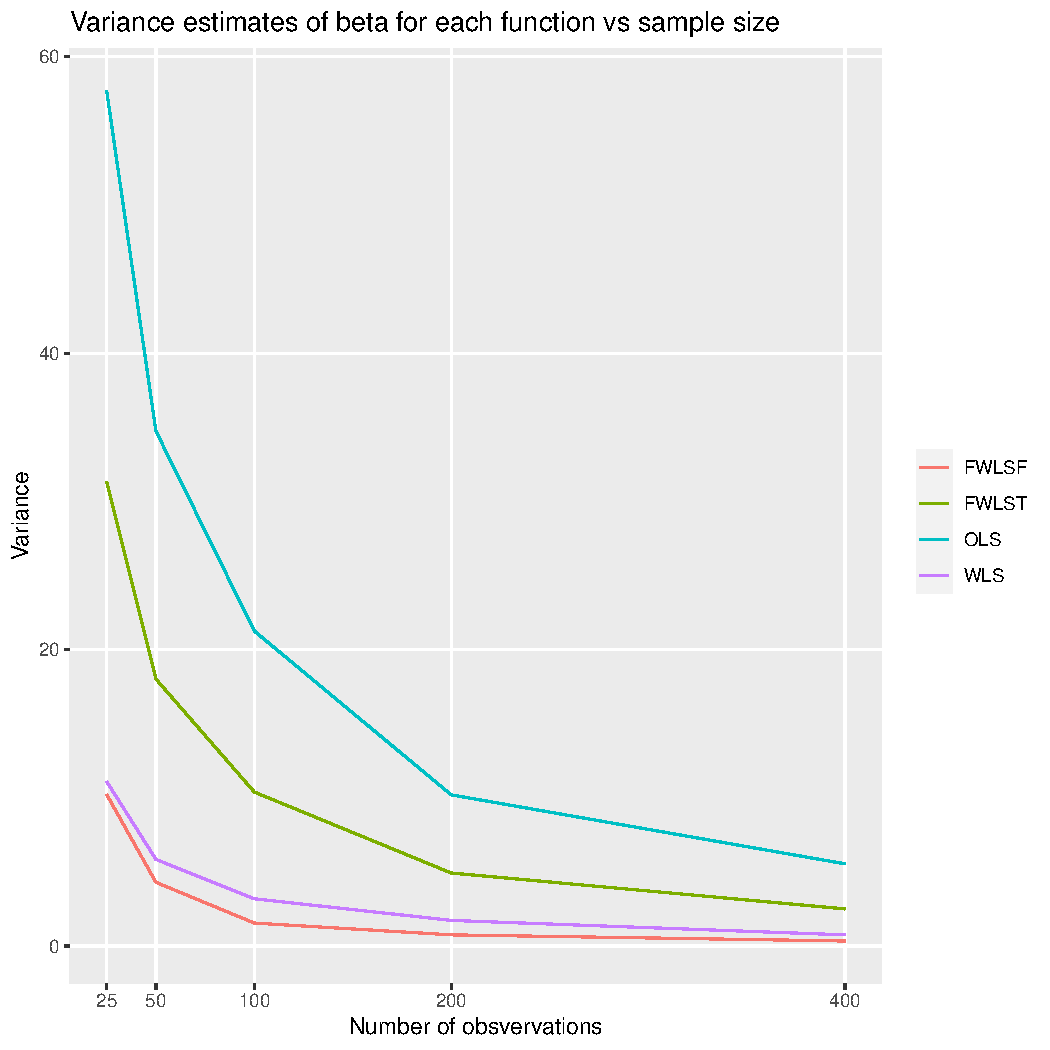
\includegraphics[width=\maxwidth]{figure/unnamed-chunk-6-1} 
\begin{kframe}\begin{alltt}
\hlcom{#############}
\end{alltt}
\end{kframe}
\end{knitrout}



\begin{knitrout}
\definecolor{shadecolor}{rgb}{0.969, 0.969, 0.969}\color{fgcolor}\begin{kframe}
\begin{alltt}
\hlcom{##################################################}
\hlcom{# start of part2}
\hlcom{##################################################}
\hlstd{galaxies} \hlkwb{<-} \hlkwd{as.data.frame}\hlstd{(galaxies)}
\hlkwd{names}\hlstd{(galaxies)} \hlkwb{<-} \hlstr{"km"}

\hlkwd{ggplot}\hlstd{(galaxies,} \hlkwd{aes}\hlstd{(}\hlkwc{x} \hlstd{= km))} \hlopt{+}
  \hlkwd{geom_density}\hlstd{()}
\end{alltt}
\end{kframe}
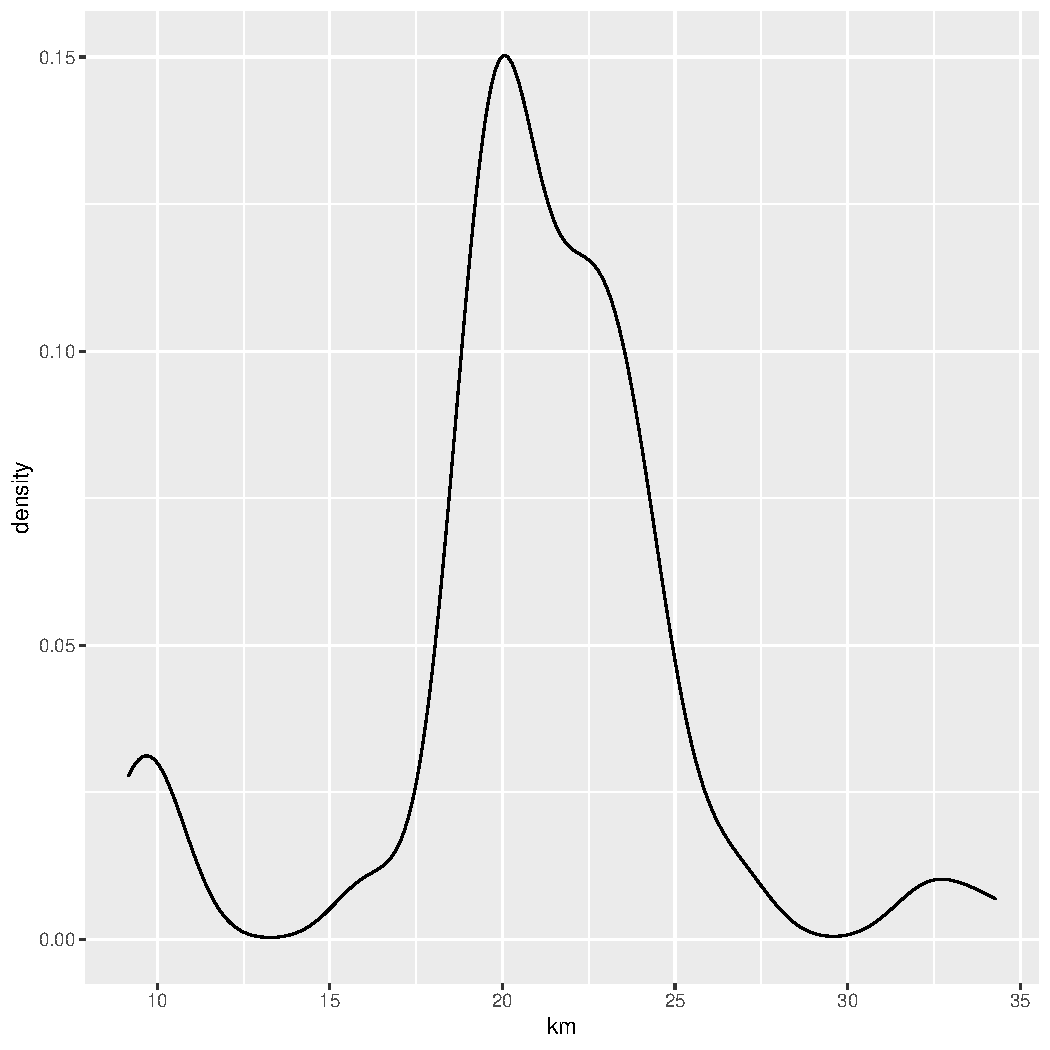
\includegraphics[width=\maxwidth]{figure/unnamed-chunk-7-1} 
\begin{kframe}\begin{alltt}
\hlstd{galaxies} \hlkwb{=} \hlstd{galaxies}\hlopt{$}\hlstd{km}

\hlstd{gammaUpdate} \hlkwb{=} \hlkwa{function}\hlstd{(}\hlkwc{x}\hlstd{,} \hlkwc{mu}\hlstd{,} \hlkwc{sigma}\hlstd{,} \hlkwc{pi}\hlstd{)\{}
  \hlstd{pdf} \hlkwb{=} \hlkwd{t}\hlstd{(}\hlkwd{sapply}\hlstd{(x, dnorm,} \hlkwc{mean} \hlstd{= mu,} \hlkwc{sd} \hlstd{= sigma))}
  \hlkwa{for}\hlstd{(n} \hlkwa{in} \hlnum{1}\hlopt{:}\hlkwd{length}\hlstd{(x))\{}
    \hlkwa{for}\hlstd{(k} \hlkwa{in} \hlnum{1}\hlopt{:}\hlkwd{length}\hlstd{(mu))\{}
      \hlstd{pdf[n, k]} \hlkwb{=} \hlstd{pi[k]}\hlopt{*}\hlstd{pdf[n, k]}
    \hlstd{\}}
  \hlstd{\}}
  \hlstd{gamma} \hlkwb{=} \hlkwd{as.data.frame}\hlstd{(}\hlkwd{matrix}\hlstd{(}\hlnum{NA}\hlstd{,} \hlkwc{ncol} \hlstd{=} \hlkwd{length}\hlstd{(pi),} \hlkwc{nrow} \hlstd{=} \hlkwd{length}\hlstd{(x)))}
  \hlkwa{for}\hlstd{(n} \hlkwa{in} \hlnum{1}\hlopt{:}\hlkwd{length}\hlstd{(x))\{}
    \hlkwa{for}\hlstd{(k} \hlkwa{in} \hlnum{1}\hlopt{:}\hlkwd{length}\hlstd{(mu))\{}
      \hlstd{gamma[n, k]} \hlkwb{=} \hlstd{pdf[n, k]}\hlopt{/}\hlkwd{sum}\hlstd{(pdf[n,])}
    \hlstd{\}}
  \hlstd{\}}
  \hlkwd{return}\hlstd{(}\hlkwd{as.data.frame}\hlstd{(gamma))}
\hlstd{\}}

\hlcom{# mu}
\hlstd{muUpdate} \hlkwb{=} \hlkwa{function}\hlstd{(}\hlkwc{x}\hlstd{,} \hlkwc{gamma}\hlstd{)\{}
  \hlstd{K} \hlkwb{<-} \hlkwd{ncol}\hlstd{(gamma)}
  \hlstd{mu} \hlkwb{<-} \hlkwa{NULL}
  \hlkwa{for} \hlstd{(i} \hlkwa{in} \hlkwd{seq_len}\hlstd{(K)) \{}
    \hlstd{mu[i]} \hlkwb{<-} \hlkwd{sum}\hlstd{(gamma[,i]}\hlopt{*}\hlstd{x)}\hlopt{/}\hlkwd{sum}\hlstd{(gamma[,i])}
  \hlstd{\}}
  \hlkwd{return}\hlstd{(mu)}
\hlstd{\}}

\hlcom{### Sigma}
\hlstd{sigmaUpdate} \hlkwb{=} \hlkwa{function}\hlstd{(}\hlkwc{x}\hlstd{,} \hlkwc{gamma}\hlstd{,} \hlkwc{mu}\hlstd{)\{}
  \hlstd{N} \hlkwb{=} \hlkwd{matrix}\hlstd{(}\hlnum{0}\hlstd{,} \hlkwc{ncol}\hlstd{=} \hlkwd{ncol}\hlstd{(gamma))}
  \hlstd{sigma} \hlkwb{=} \hlkwd{matrix}\hlstd{(}\hlnum{0}\hlstd{,} \hlkwc{ncol} \hlstd{=} \hlkwd{ncol}\hlstd{(gamma))}
  \hlkwa{for}\hlstd{(k} \hlkwa{in} \hlnum{1}\hlopt{:}\hlkwd{ncol}\hlstd{(gamma))\{}
    \hlkwa{for}\hlstd{(n} \hlkwa{in} \hlnum{1}\hlopt{:}\hlkwd{length}\hlstd{(x))\{}
      \hlstd{sigma[k]} \hlkwb{=} \hlstd{sigma[k]} \hlopt{+} \hlstd{gamma[n,k]}\hlopt{*}\hlstd{(x[n]}\hlopt{-}\hlstd{mu[k])}\hlopt{^}\hlnum{2}
      \hlstd{N[k]} \hlkwb{=} \hlstd{N[k]} \hlopt{+} \hlstd{gamma[n,k]}
    \hlstd{\}}
    \hlstd{sigma[k]} \hlkwb{=} \hlkwd{sqrt}\hlstd{(sigma[k]}\hlopt{/}\hlstd{N[k])}
  \hlstd{\}}
  \hlkwd{return}\hlstd{(sigma)}
\hlstd{\}}

\hlstd{piUpdate} \hlkwb{=} \hlkwa{function}\hlstd{(}\hlkwc{gamma}\hlstd{)\{}
  \hlstd{pi} \hlkwb{<-} \hlkwa{NULL}
  \hlkwa{for} \hlstd{(i} \hlkwa{in} \hlnum{1}\hlopt{:}\hlkwd{ncol}\hlstd{(gamma)) \{}
    \hlstd{pi[i]} \hlkwb{<-} \hlkwd{sum}\hlstd{(gamma[,i])}\hlopt{/}\hlkwd{sum}\hlstd{(gamma)}
  \hlstd{\}}
  \hlkwd{return}\hlstd{(pi)}
\hlstd{\}}

\hlcom{### Log-likelihood }
\hlstd{loglik} \hlkwb{=} \hlkwa{function}\hlstd{(}\hlkwc{x}\hlstd{,} \hlkwc{pi}\hlstd{,} \hlkwc{mu}\hlstd{,} \hlkwc{sigma}\hlstd{)\{}
  \hlstd{sum_pdf} \hlkwb{=} \hlkwd{matrix}\hlstd{(}\hlnum{0}\hlstd{,} \hlkwc{nrow} \hlstd{=} \hlkwd{length}\hlstd{(x))}
  \hlstd{loglike} \hlkwb{=} \hlnum{0}
  \hlkwa{for}\hlstd{(n} \hlkwa{in} \hlnum{1}\hlopt{:}\hlkwd{length}\hlstd{(x))\{}

    \hlkwa{for}\hlstd{(k} \hlkwa{in} \hlnum{1}\hlopt{:}\hlkwd{length}\hlstd{(pi))\{}
      \hlstd{sum_pdf[n]} \hlkwb{=} \hlstd{sum_pdf[n]} \hlopt{+} \hlstd{(pi[k]} \hlopt{*} \hlkwd{dnorm}\hlstd{(x[n], mu[k], sigma[k]))}
    \hlstd{\}}
    \hlstd{loglike} \hlkwb{=} \hlstd{loglike} \hlopt{+} \hlkwd{log}\hlstd{(sum_pdf[n])}
  \hlstd{\}}
  \hlkwd{return}\hlstd{(loglike)}
\hlstd{\}}

\hlstd{initialValues} \hlkwb{=} \hlkwa{function}\hlstd{(}\hlkwc{x}\hlstd{,} \hlkwc{K}\hlstd{,} \hlkwc{reps} \hlstd{=} \hlnum{100}\hlstd{)\{}
  \hlstd{mu} \hlkwb{=} \hlkwd{rnorm}\hlstd{(K,} \hlkwd{mean}\hlstd{(x),} \hlnum{5}\hlstd{)}
  \hlstd{sigma} \hlkwb{=} \hlkwd{sqrt}\hlstd{(}\hlkwd{rgamma}\hlstd{(K,} \hlnum{5}\hlstd{))}
  \hlstd{p} \hlkwb{=} \hlkwd{runif}\hlstd{(K)}
  \hlstd{p} \hlkwb{=} \hlstd{p}\hlopt{/}\hlkwd{sum}\hlstd{(p)}
  \hlstd{currentLogLik} \hlkwb{=} \hlkwd{loglik}\hlstd{(x, p, mu, sigma)}
  \hlkwa{for}\hlstd{(i} \hlkwa{in} \hlnum{1}\hlopt{:}\hlstd{reps)\{}
    \hlstd{mu_temp} \hlkwb{=} \hlkwd{rnorm}\hlstd{(K,} \hlkwd{mean}\hlstd{(x),} \hlnum{10}\hlstd{)}
    \hlstd{sigma_temp} \hlkwb{=} \hlkwd{sqrt}\hlstd{(}\hlkwd{rgamma}\hlstd{(}\hlnum{10}\hlstd{,} \hlnum{5}\hlstd{))}
    \hlstd{p_temp} \hlkwb{=} \hlkwd{runif}\hlstd{(K)}
    \hlstd{p_temp} \hlkwb{=} \hlstd{p_temp}\hlopt{/}\hlkwd{sum}\hlstd{(p_temp)}
    \hlstd{tempLogLik} \hlkwb{=} \hlkwd{loglik}\hlstd{(x, p_temp, mu_temp, sigma_temp)}
    \hlkwa{if}\hlstd{(tempLogLik} \hlopt{>} \hlstd{currentLogLik)\{}
      \hlstd{mu} \hlkwb{=} \hlstd{mu_temp}
      \hlstd{sigma} \hlkwb{=} \hlstd{sigma_temp}
      \hlstd{p} \hlkwb{=} \hlstd{p_temp}
      \hlstd{currentLogLik} \hlkwb{=} \hlstd{tempLogLik}
    \hlstd{\}}
  \hlstd{\}}
  \hlkwd{return}\hlstd{(}\hlkwd{list}\hlstd{(}\hlstr{"mu"} \hlstd{= mu,} \hlstr{"sigma"} \hlstd{= sigma,} \hlstr{"p"} \hlstd{= p))}
\hlstd{\}}

\hlcom{##################################################}
\hlcom{# EM algo}
\hlcom{##################################################}
\hlstd{EM} \hlkwb{=} \hlkwa{function}\hlstd{(}\hlkwc{x}\hlstd{,} \hlkwc{K}\hlstd{,} \hlkwc{tol} \hlstd{=} \hlnum{0.001}\hlstd{)\{}
  \hlstd{inits} \hlkwb{=} \hlkwd{initialValues}\hlstd{(x, K,} \hlnum{1000}\hlstd{)}
  \hlstd{mu} \hlkwb{=} \hlstd{inits}\hlopt{$}\hlstd{mu}
  \hlstd{sigma} \hlkwb{=} \hlstd{inits}\hlopt{$}\hlstd{sigma}
  \hlstd{prob} \hlkwb{=} \hlstd{inits}\hlopt{$}\hlstd{p}

  \hlstd{prevLoglik} \hlkwb{<-} \hlnum{0}
  \hlstd{loglikDiff}\hlkwb{<-} \hlnum{1}

  \hlcom{# while loop}
  \hlkwa{while}\hlstd{(loglikDiff} \hlopt{>} \hlstd{tol)\{}

    \hlstd{gamma} \hlkwb{<-} \hlkwd{gammaUpdate}\hlstd{(x, mu, sigma, prob)}
    \hlstd{mu} \hlkwb{<-} \hlkwd{muUpdate}\hlstd{(x, gamma)}
    \hlstd{sigma} \hlkwb{<-} \hlkwd{sigmaUpdate}\hlstd{(x, gamma, mu)}
    \hlstd{prob} \hlkwb{<-} \hlkwd{piUpdate}\hlstd{(gamma)}

    \hlstd{currentLogLik} \hlkwb{<-} \hlkwd{loglik}\hlstd{(x, prob, mu, sigma)}

    \hlstd{loglikDiff} \hlkwb{<-} \hlkwd{abs}\hlstd{(prevLoglik} \hlopt{-} \hlstd{currentLogLik)}

    \hlstd{prevLoglik} \hlkwb{<-} \hlstd{currentLogLik}

  \hlstd{\}}

  \hlkwd{return}\hlstd{(}\hlkwd{list}\hlstd{(}\hlstr{'loglik'} \hlstd{= currentLogLik,} \hlstr{'mu'} \hlstd{= mu,} \hlstr{'sigma'} \hlstd{= sigma,} \hlstr{'prob'} \hlstd{= prob))}
\hlstd{\}}

\hlkwd{set.seed}\hlstd{(}\hlnum{1996}\hlstd{)}
\hlstd{final_plot} \hlkwb{=} \hlkwd{matrix}\hlstd{(}\hlnum{0}\hlstd{,} \hlkwc{ncol} \hlstd{=} \hlnum{4}\hlstd{,} \hlkwc{nrow}\hlstd{=} \hlkwd{length}\hlstd{(galaxies))}
\hlstd{loglik_values} \hlkwb{=} \hlkwa{NULL}
\hlkwa{for}\hlstd{(k} \hlkwa{in} \hlnum{2}\hlopt{:}\hlnum{5}\hlstd{)\{}
  \hlstd{z} \hlkwb{=} \hlkwd{EM}\hlstd{(galaxies, k)}
  \hlstd{loglik_values[(k}\hlopt{-}\hlnum{1}\hlstd{)]} \hlkwb{=} \hlstd{z}\hlopt{$}\hlstd{loglik}
  \hlkwa{for}\hlstd{(i} \hlkwa{in} \hlnum{1}\hlopt{:}\hlstd{k)\{}
    \hlstd{final_plot[,(k}\hlopt{-}\hlnum{1}\hlstd{)]} \hlkwb{=} \hlstd{final_plot[,(k}\hlopt{-}\hlnum{1}\hlstd{)]} \hlopt{+} \hlstd{z}\hlopt{$}\hlstd{prob[i]} \hlopt{*} \hlkwd{dnorm}\hlstd{(galaxies, z}\hlopt{$}\hlstd{mu[i], z}\hlopt{$}\hlstd{sigma[i])}
  \hlstd{\}}
\hlstd{\}}

\hlstd{loglik_values} \hlkwb{<-} \hlkwd{as.data.frame}\hlstd{(loglik_values)} \hlopt
  \hlkwd{mutate}\hlstd{(}\hlstr{"K"} \hlstd{= (}\hlnum{2}\hlopt{:}\hlnum{5}\hlstd{))}
\end{alltt}


{\ttfamily\noindent\bfseries\color{errorcolor}{\#\# Error in as.data.frame(loglik\_values) \%>\% mutate(K = (2:5)): could not find function "{}\%>\%"{}}}\begin{alltt}
\hlstd{loglik_plot} \hlkwb{=} \hlkwd{ggplot}\hlstd{(}\hlkwc{data} \hlstd{= loglik_values)} \hlopt{+}
  \hlkwd{geom_line}\hlstd{(}\hlkwd{aes}\hlstd{(}\hlkwc{x}\hlstd{=K,} \hlkwc{y}\hlstd{=loglik_values),} \hlkwc{color} \hlstd{=} \hlstr{"blue"}\hlstd{)} \hlopt{+}
  \hlkwd{labs}\hlstd{(}\hlkwc{x}\hlstd{=}\hlstr{"Number of components"}\hlstd{,}\hlkwc{y}\hlstd{=} \hlstr{"Log likelihood"}\hlstd{)}
\end{alltt}


{\ttfamily\noindent\bfseries\color{errorcolor}{\#\# Error: `data` must be a data frame, or other object coercible by `fortify()`, not a numeric vector}}\begin{alltt}
\hlstd{final_plot} \hlkwb{=} \hlkwd{as.data.frame}\hlstd{(final_plot)}
\hlkwd{colnames}\hlstd{(final_plot)} \hlkwb{=} \hlkwd{c}\hlstd{(}\hlstr{"K = 2"}\hlstd{,} \hlstr{"K = 3"}\hlstd{,} \hlstr{"K = 4"}\hlstd{,} \hlstr{"K = 5"}\hlstd{)}
\hlstd{final_plot} \hlkwb{=} \hlkwd{cbind}\hlstd{(final_plot, galaxies)}

\hlkwd{ggplot}\hlstd{(}\hlkwc{data} \hlstd{= final_plot,} \hlkwd{aes}\hlstd{(}\hlkwc{x} \hlstd{= galaxies))} \hlopt{+}
  \hlkwd{geom_line}\hlstd{(}\hlkwd{aes}\hlstd{(}\hlkwc{y} \hlstd{= `K = 2`,} \hlkwc{color} \hlstd{=} \hlstr{"K = 2"}\hlstd{),} \hlkwc{size} \hlstd{=} \hlnum{1}\hlstd{)} \hlopt{+}
  \hlkwd{geom_line}\hlstd{(}\hlkwd{aes}\hlstd{(}\hlkwc{y} \hlstd{= `K = 3`,} \hlkwc{color} \hlstd{=} \hlstr{"K = 3"}\hlstd{),} \hlkwc{size} \hlstd{=} \hlnum{1}\hlstd{)} \hlopt{+}
  \hlkwd{geom_line}\hlstd{(}\hlkwd{aes}\hlstd{(}\hlkwc{y} \hlstd{= `K = 4`,} \hlkwc{color} \hlstd{=} \hlstr{"K = 4"}\hlstd{),} \hlkwc{size} \hlstd{=} \hlnum{1}\hlstd{)} \hlopt{+}
  \hlkwd{geom_line}\hlstd{(}\hlkwd{aes}\hlstd{(}\hlkwc{y} \hlstd{= `K = 5`,} \hlkwc{color} \hlstd{=} \hlstr{"K = 5"}\hlstd{),} \hlkwc{size} \hlstd{=} \hlnum{1}\hlstd{)} \hlopt{+}
  \hlkwd{geom_density}\hlstd{(}\hlkwd{aes}\hlstd{(}\hlkwc{fill} \hlstd{=} \hlstr{"Density plot"}\hlstd{),} \hlkwc{color} \hlstd{=} \hlstr{"pink"}\hlstd{,} \hlkwc{alpha} \hlstd{=} \hlnum{0.2}\hlstd{,} \hlkwc{size} \hlstd{=} \hlnum{0}\hlstd{)} \hlopt{+}
  \hlkwd{labs}\hlstd{(}\hlkwc{x} \hlstd{=} \hlstr{"km"}\hlstd{,} \hlkwc{y} \hlstd{=} \hlstr{"Density"}\hlstd{,}\hlkwc{title}\hlstd{=}\hlstr{"Plot of different values of K and the density plot of galaxies"}\hlstd{)} \hlopt{+}
  \hlkwd{theme}\hlstd{(}\hlkwc{legend.title} \hlstd{=} \hlkwd{element_blank}\hlstd{(),}\hlkwc{legend.position} \hlstd{=} \hlkwd{c}\hlstd{(}\hlnum{.95}\hlstd{,} \hlnum{.95}\hlstd{),}
        \hlkwc{legend.justification} \hlstd{=} \hlkwd{c}\hlstd{(}\hlstr{"right"}\hlstd{,} \hlstr{"top"}\hlstd{),}
        \hlkwc{legend.box.just} \hlstd{=} \hlstr{"right"}\hlstd{,}
        \hlkwc{legend.margin} \hlstd{=} \hlkwd{margin}\hlstd{(}\hlnum{6}\hlstd{,} \hlnum{6}\hlstd{,} \hlnum{6}\hlstd{,} \hlnum{6}\hlstd{))}
\end{alltt}
\end{kframe}
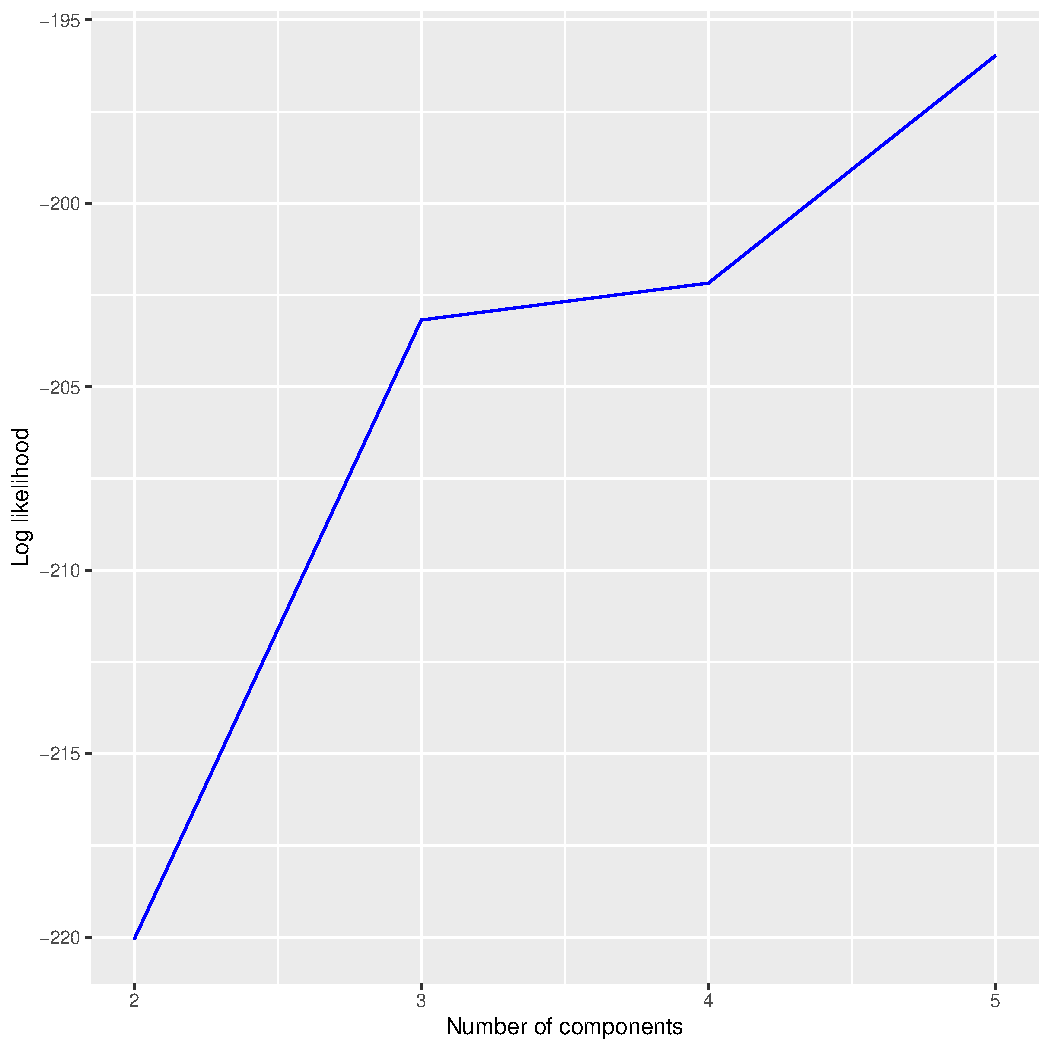
\includegraphics[width=\maxwidth]{figure/unnamed-chunk-7-2} 

\end{knitrout}

